\documentclass{bioinfo}
\copyrightyear{2005}
\pubyear{2005}

\begin{document}
\firstpage{1}

\title[Application Note]{bioWeb3D a simple online webGL 3D data visualization tool}
\author[Sample \textit{et~al}]{Jean-Baptiste Pettit\,$^{1,*}$ and John Marioni\,$^{1}$\footnote{to whom correspondence should be addressed}}
\address{$^{1}$Department of XXXXXXX, Address XXXX etc.\\
$^{1}$European Bioinformatics Institute}

\history{Received on XXXXX; revised on XXXXX; accepted on XXXXX}

\editor{Associate Editor: XXXXXXX}

\maketitle

\begin{abstract}

\section{Summary:}
An online HTML5/webGL based 3D visualization tool has been developed to allow biologists to quickly and simply view interactive and customizable three dimensional representations of their data along with multiple layers of information. Using the WebGL library Three.js written in Javascript, bioWeb3D allows the simultaneous visualization of multiple large datasets input through a simple JSON file, read and analysed locally thanks to HTML5 capabilities.

\section{Availability:}
http://ebi.ac.uk/~jbpettit/bioWeb3D \\ https://github.com/jibooo/bio3D

\section{Contact:} \href{jbpettit@ebi.ac.uk}{jbpettit@ebi.ac.uk}
\end{abstract}

\section{Introduction}

Large biological datasets analysis is helped to a great extent by visualization when analysing organized structures especially when it comes to clustering results \citep{Rubel10}. In many fields now, 3D datasets are generated. Some visualization software have been developed, but always through a local install software like Arena3D \citep{Pavlopoulos08},  3D Genome Tuner \citep{Wang09}, the Allen Brain Atlas \citep{Lein07} or Cytoscape \citep{Shannon03} with a specific plug-in. Other 3D visualization tools are built online and accessible through the browser directly, for proteins 3D structures visualization for example Astexviewer \citep{Hartshorn02} on the Protein Databank Europe using Java Applets. More recently the first applications using HTML5/WebGL capabilities were published for very specific use cases such as radiology information \citep{Dinesh12} but never before has a tool allowed biologists to view potentially any kind of 3D data directly online in an easy, fast, secure and interactive way. Using webGL and HTML5 3D capabilities and wide range availability, bioWeb3D aims to be a simple non specialized tool for data and information overview.



\section{Technological overview}

bioWeb3D allows the representation of any 3D dataset by defining two file formats enabling users to input quickly their own datasets in the application. The format is based on JSON, a widely used structured format on the web.\\
The first file type carries the coordinates of all the points in the dataset while the second describes one or several information layer about the previously defined points.\\
Datasets can be viewed and compared in up to four worlds at the same time. We call information layer the characteristics attached to the points defined in the dataset or in other words a classification of the data points in different classes.  Although web based, the application fully written in Javascript does not need to send any data to the host server. To this end the modern browsers local file system reading capabilities are used through the HTML 5 FileReader functionality. This allows the application to handle in a very short time large datasets while remaining entirely safe for the user privacy. \\
Although aimed to remain very simple and easy to use, some options are available for the user to customize the way their datasets are represented. The application can be used to visualize sequential information such as 3D protein structure in which case links can be drawn between the points. In other cases, the points can be left unlinked as individual particles. \\
The way the information layers are shown in the visualization is by colouring the 3D points with regard to which class each point belongs.\\
\subsection{Defining the input files format}
The JSON format has been chosen for its rigorous structure allowing fast Javascript objects generation within the browser interpreter. Compared to other data-interchange language such as XML, JSON is also easily human readable thanks to a light-weight syntax. It is also supported by all the main internet browsers on the market.\\
The dataset file root object must be called "dataset" and contains :
\begin{itemize}
\item The "name" property of the dataset
\item The "points" property which is a two dimensional array representing a list of (x,y,z) vectors defining the points coordinates.
\end{itemize}

The information layer files have to have their root element named  "cluster". Because one information file can define multiple information sets, the structure below "cluster" is a list. Each element of the list is structured as follow :
\begin{itemize}
\item The "name" property (optional)
\item The "numClust" property which indicates the number of different classes the data will be assigned to.
\item The "labels" property which defines a list of names for the "numClust" classes previously defined (optional)
\item The values property which defines the class of each point in the dataset. As points don't have single IDs, this property must be in the same order and have the same length than the points defined in the dataset file.
\end{itemize}
Exact specifications and examples of the file formats can be found on the BioWeb3D gitHub repository's wiki. Because many biological results are in fact stored as CSV files we also provide easy to use Perl scripts designed to quickly generate JSON files from CSV data. You can find those scripts in the GitHub repository.


\begin{figure}[h!]%figure1
\centerline{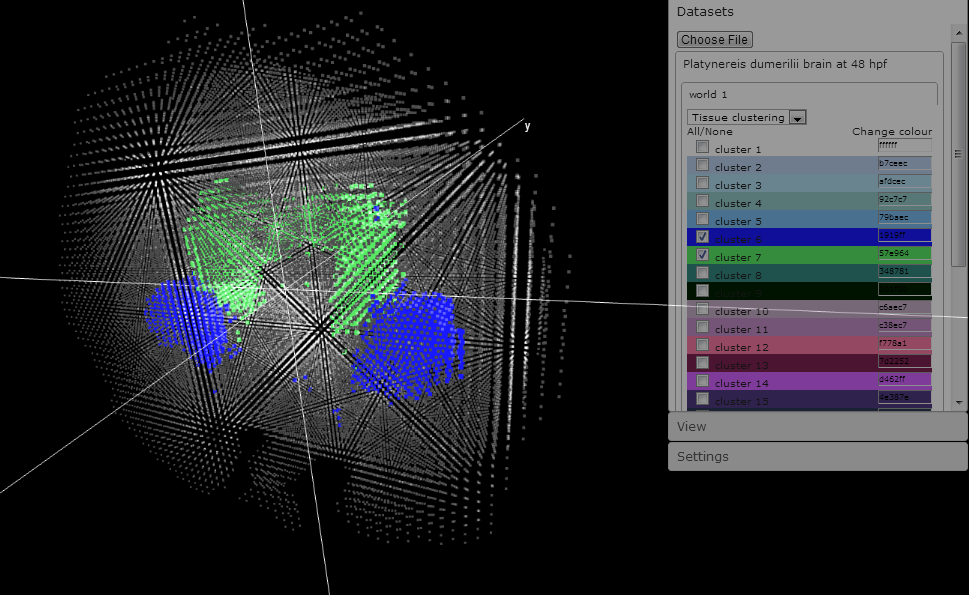
\includegraphics[totalheight=0.2\textheight]{fig1.png}}
\caption{left:Marine annelid Platynereis dumerilii single cell clustering results. Two clusters are shown along with the shadow of the remaining cells. right: Main carbon chain structure of a Bacterial pentameric ligand-gated ion channel, in red the $\alpha$-helix are highlighted in green the $\beta$-sheets. The User interface is visible on the right of the screen and can be hidden with the "show/hide" button located on the bottom left}\label{fig:01}
\end{figure}

\subsection{User interface}
The user can interact with the visualization via an interface on the right of the screen. Three panels are available, in the "dataset" panel, the user can register the input files and chose which datasets and information layers should be represented in which world, this panel also allows to show/hide specific classes of the selected information layers. Each dataset file entered will create a new sub-panel from which he user can input the information files creating new options in a drop-down list for each world. Selecting one information layer in the drop-down list will show the data in the current world and populate a list of classes that the user will be able to modify regarding their visibility and colour.\\
The "View" panel enables the user to choose which of the worlds are shown on the screen, ranging from 1 to 4 simultaneous worlds.
Finally the "Settings" panel provides the user with a few options affecting all the worlds and all the datasets. Namely it allows to modify the axes scales.


\section{Discussion}
	\subsection{bioWeb3D and local software}
Many 3D visualization software exist and provide similar functionalities with standard 3D format input such as .OBJ, some are extremely generic and powerful but have a steep learning curve like Blender. Those are not usually oriented towards science specifically. Others are science oriented but very specific to a type of data especially in medical sciences \citep{Wang09}. In this context we believe that bioWeb3D can be useful as it is completely generic and web based. It should also be noted that recent browsers improvements regarding GPU acceleration through the webGL paradigm allow bioWeb3D to visualize several hundred thousand three dimensional data points and to interact with then with a perfect fluidity even on a laptop competing directly in that sense with local software. Local software are usually platform specific, which is not the case for web based applications.

	\subsection{bioWeb3D and Java Applets}
As mentioned before web based 3D visualization tools exists mainly in the form of Java Applets. This technology has attracted much criticism in 2012 regarding security flaws, leading the "United States Computer Emergency Readiness Team" to advise to disable Java Applets altogether for current and future Java vulnerabilities \citep{USCERT12}. The developpement of WebGL technology is viewed by many as a candidate replacement for Applets. 

	\subsection{Current limits}
The main limitation of a webGl based application in 2012 is the machine and browser compatibility. Only computers with fairly recent graphic cards will be able to run a 3D environment. It should also be noted that if Microsoft has notify the developer community that Internet Explorer was scheduled to support WebGL, both Chrome and Firefox now fully support webGL applications.



\section*{Acknowledgement}
The authors would like to acknowledge Ricardo Cabello (also known as Mrdoob), Samuel Croset, Tom Oldfield and Sergio Martinez Cuesta for their precious contributions to the project.



\begin{thebibliography}{}
\bibitem[Shannon {\it et~al}., 2003]{Shannon03} Shannon P, Markiel A, Ozier O, Baliga NS, Wang JT, Ramage D, Amin N, Schwikowski B, Ideker T (2003) Cytoscape: a software environment for integrated models of biomolecular interaction networks., {\it Genome Res}, {\bf 13(11)}, 12498-2504.

\bibitem[Wang {\it et~al}., 2009]{Wang09} Qi Wanga, Qun Lianga, Xiuqing Zhanga (2009) 3D Genome Tuner: Compare Multiple Circular Genomes in a 3D Context., {\it Genomics, Proteomics and Bioinformatics}, {\bf 7(3)}, 143–146.

\bibitem[Pavlopoulos {\it et~al}., 2008]{Pavlopoulos08} Georgios A Pavlopoulos, Seán I O'Donoghue, Venkata P Satagopam, Theodoros G Soldatos, Evangelos Pafilis and Reinhard Schneider (2008) Arena3D: visualization of biological networks in 3D., {\it BMC Systems Biology}, {\bf 2(104)}.

\bibitem[Dinesh {\it et~al}., 2012]{Dinesh12} Dinesh B. KulkarniMahesh M. DoijadeChetan S. DevrukhkarGanesh R. ZilpeRajesh R. Surana (2012) NetraRIS - a Web based DICOM Viewer., {\it International Journal of Computer Applications}, {\bf 48(24)}.

\bibitem[Lein {\it et~al}., 2007]{Lein07} Lein ES, Hawrylycz MJ, Ao N, Ayres M, Bensinger A, Bernard A, Boe AF, Boguski MS, Brockway KS, Byrnes EJ, Chen L, Chen L, Chen TM, Chin MC, Chong J, Crook BE, Czaplinska A, Dang CN, Datta S, Dee NR, et al (2007) Genome-wide atlas of gene expression in the adult mouse brain., {\it Nature}, {\bf 445}, 168–176.


\bibitem[Hartshorn, 2002]{Hartshorn02} Hartshorn (2002) Astex Technology Ltd., 436 Cambridge Science Park, Milton Road, Cambridge, CB5 9QA, UK. m.hartshorn@astex-technology.com.

\bibitem[Oracle, 2012]{Oracle12} Oracle (2012) Oracle Security Alert for CVE-2012-4681, {\it http://www.oracle.com/technetwork/topics/security/alert-cve-2012-4681-1835715.html}.

\bibitem[Rubel {\it et~al}., 2010]{Rubel10} Rubel O, Weber GH, Huang MY, Bethel EW, Biggin MD, Fowlkes CC, Luengo Hendriks CL, Keränen SV, Eisen MB, Knowles DW, Malik J, Hagen H, Hamann B (2010)Integrating Data Clustering and Visualization for the Analysis of 3D Gene Expression Data., {\it IEEE/ACM Trans Comput Biol Bioinform}, {\bf 7(1)}.

\bibitem[US-CERT, 2012]{USCERT12} Oracle (2012) United States Computer Emergency Readiness Team, {\it http://www.kb.cert.org/vuls/id/636312}.




\end{thebibliography}
\end{document}
